% !TeX spellcheck = en_US
% !TeX root = DynELA.tex
%
% LaTeX source file of DynELA FEM Code
%
% (c) by Olivier Pantalé 2020
%
\chapter{History of the \DynELA}\label{Chapter!History}

\startcontents[chapters]
\printmyminitoc[1]\LETTRINE{T}he \DynELA, currently in its $4^{th}$ version, is a project for the development of an explicit dynamic Finite Element code in large deformations started in 1996, following my thesis work on the development of a numerical model for the simulation of metal cutting, carried out by an Arbitrary Eulero-Lagrangian (ALE) approach on the Radioss simulation code. Following this thesis work, during which some numerical developments have focused on the realization of an interactive graphical post-processor for the analysis of the results of simulations with the Radioss calculation code, it was decided to develop an Explicit FEM code in Large Deformations, initially as a simple project of initiation to programming. Subsequently, these developments having shown an interest, it was decided to continue them and to improve little by little the capacities of this laboratory FEM code.

\section{The first version of the FEM code}
The first versions of the \DynELA (from v.1.0 to v.3.0) were mainly developed from 1996 to 2010.
\begin{itemize}
\item Elements and material library:
\subitem 2D triangles and quadrangles, axisymmetric
\subitem 3D tetrahedrons and hexahedrons
\subitem Elasticity, $J_{2}$ plasticity, Elastoplastic flow law
\item Numerical Solvers:
\subitem Explicit integration scheme (Chung-Hulbert)
\subitem Domain Decomposition Method (spatial and temporal)
\subitem Parallel computing with OpenMP
\subitem X-FEM support
\item Environment and usage:
\subitem Interfaces to Abaqus FEM code (read and write)
\subitem High level language script (like Python)
\subitem Graphic User Interface (see Figure \ref{fig:History!DynELAv1})
\subitem Parametric language and automatic extraction of results
\end{itemize}

The DynELA v.1 to v.3 FEM code is written in \Cpp and consist of about 150.000 lines of code. This previous version has been included into the CAE Linux distribution some year ago and the corresponding work has been published in some Scientific Journals \cite{
pantale_object-oriented_2002,
pantale_development_2004,
pantale_parallelization_2005,
menanteau_methodology_2006,
nistor_numerical_2007,
nistor_numerical_2008,
pantale_rp_2020}
, some international conferences \cite{
menanteau_coupled_2005,
nistor_modeling_2005,
pantale_strategies_2005,
pantale_developpement_2004,
pantale_developpement_1999,
pantale_development_2002}
 and served to support for some Ph.D. theses \cite{
menanteau_developpement_2004,
nistor_identification_2005}
. The FEM code includes a numerical core solver, a high level language script based on the use of the Flex and Bison unix tools for grammar and syntax analysis.

\begin{figure}[h]
\begin{centering}
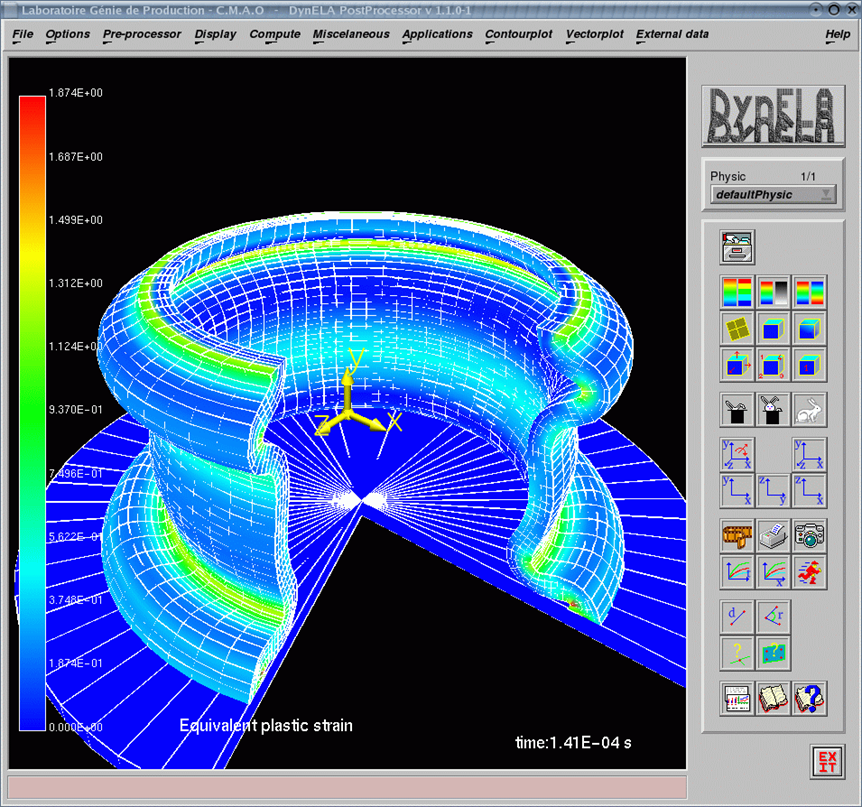
\includegraphics[width=0.5\columnwidth]{Figures/DynELA-v.1.1}
\par\end{centering}
\caption{GUI interface of the DynELA v.1.0 FEM code\label{fig:History!DynELAv1}}
\end{figure}

\section{The new version of the FEM code}
The new version of the code is mainly written in \Cpp and Python, and the aim of this new v.4.0 is to provide an enhanced version of the code with enhancements concerning the constitutive laws, a new programming interface based on Python 3 formalism, along with some enhanced documentation.

The Graphics User Interface reported in Figure \ref{fig:History!DynELAv1} and based on OpenGL and QT has been abandoned in this new version. The high level script language based on the use of Flex and Bison tools has also been abandoned and replaced by an interface based on Python's 3 language with the use of the SWIG tool to create the interface between \Cpp classes and Python 3.
